
\section*{Lecture 8 (27.04.2016}
\subsection*{Discete Choice Modelle}

Messung/Daten: Paarweise Präferenzen auf endliche Menge A\\

$a \geq b \Leftrightarrow u_a \geq u_b$, wobei $u_a = v_a+ \epsilon_a$\\
$v_a$ ist dabei deterministisch\\
$\epsilon_A$ ist das prob. Rauschen\\

\begin{center}


\begin{tabular}{r l}
$P_r[u_a \geq u_b]$&$ = P_r[v_a + \epsilon_a \geq v_b + \epsilon_b]$\\
&$ = P_r[v_a -v_b \geq \epsilon_b - \epsilon_a]$\\
&$ = P_r[\underbrace{\epsilon_b - \epsilon_a}_{Zufallsvariable} \leq \underbrace{v_a -v_b}_{Wert} ]$
\end{tabular}
\end{center}


\underline{Zwei Modelle:} 
\begin{enumerate}
\item \textbf{Thurstone/Probit:}\\ $v_a - v_b = \sqrt{s \sigma} \Phi^{-1}(P_{ab})$\\$v_{ab} := \sqrt{2\phi} \Phi^{-1}(f_{ab})$

\item \textbf{Bradley-Terry/Logit:} \\$v_a - v_b = \log(\frac{P_{ab}}{1-P_{ab}})$\\$v_{ab} := log(\frac{f_{ab}}{1-f_{ab}})$

\end{enumerate}

Problem: Wir haben den Schätzwert für $v_{ab}$, brauchen aber den Schätzwert für die $v_a$.\newline\newline

Zur Bestimmung von den $v_a$ aus den $v_{ab}$, definieren wir eine \textbf{Loss-Funktion} (ein bisschen hacky).

$$L(v_a | a \in A) = \dfrac{1}{2} \sum_{a \in A}\sum_{\underset{b \neq a}{b \in A}}((v_a - v_b)-(v_{ab}))^2$$
Wir minimieren die quadratiche Abweichung um den Loss zu minimieren.\\
\textbf{Ziel:} Bestimme $v_a$ so, dass der Loss minimiert ist. Notwendig für den Minimum des Losses ist das verschwinden des Gradienten.

$$\bigtriangledown_{v_a}L(v_a) =  \sum_{b \in A}(v_a - v_b - v_{ab}) \overset{!}{=} 0$$
$$\Rightarrow  \sum_{b \in A}v_b + \sum_{\underset{b \neq a}{b \in A}}v_{ab} = v_a |A|$$

\underline{Annahme:} \\$ \sum_{b \in A}v_b = 0$ [entspricht einer Verschiebung aller $v_b$, hat keinen Effekt auf die Ordnung der $v_b$]\\
$$\Rightarrow v_a = \dfrac{1}{|A|} \sum_{\underset{b \neq a}{b \in A}} v_{ab}$$

Einsetzen der Schätzwerte für $v_{ab}$ ergibt:
\begin{enumerate}
\item \textbf{Thurstone/Probit:}\\
\framebox[1.3\width]{$v_a = \dfrac{\sqrt{2\sigma}}{|A|}\sum_{\underset{b \neq a}{b \in A}}\Phi^{-1}(f_{ab})$}



\item \textbf{Bradley-Terry/Logit:}\\
\framebox[1.3\width]{$v_{a} := \frac{1}{|A|}\sum_{\underset{b \neq a}{b \in A}}log(\frac{f_{ab}}{1-f_{ab}})$}


\end{enumerate}

\subsection*{Bias-Varianz Tradeoff (Regression)}
Modell: \framebox[1.3\width]{$y = f(x)+\epsilon$}\\
Daten: $(x^{(1)},y^{(1)}),...,(x^{(n)},y^{(n)})$\\
\begin{enumerate}
\item Variate   $y \in \mathbb{R}$
\item Covariates    $x \in \mathbb{R}^n$
\item $f: \mathbb{R}^n \rightarrow \mathbb{R} =$ eine deterministische Funktion
\item $\epsilon$ ist das Rauschen, so dass:
\begin{itemize}
\item $E[\epsilon] = 0$
\item $Var(\epsilon) = \sigma^2$
\end{itemize}
\end{enumerate}
Aus den Daten lernen wir das Modell $\hat{f} bzw \hat{f}(x)$ sind zufällige Größen.\\
\textbf{Frage:} Wie gut ist unser Modell? Dazu betrachten wir den erwarteten quadratischen Fehler.
$$E[(y-\hat{f}(x_0))^2 | x = x_0] $$
$$= E[(y-E[\hat{f}(x_0)] + E[\hat{f}(x_0)] - \hat{f}(x_0)^2 | x = x_0] $$
$$= E[(y-E(\hat{f}(x_0)^2] + 2E[
\underbrace{
\underbrace{(y-\hat{f}(x_0))}_{hier: y = zufällig}(\underbrace{E[\hat{f}(x_0)]-\hat{f}(x_0))}_{hier: f(x_0) = zufällig}}_{2E[(y-\hat{f}(x_0))] | x = x_0] \cdot \underbrace{E[E[\hat{f}(x_0)]-\hat{f}(x_0)]}_{=0}} | x = x_0] + E[E[\hat{f}(x_0)]-\hat{f}(x_0)^2]$$
\todo{das soll jemand checken}
$$= E[(y-E[\hat{f}(x_0)]J)^2  | x = x_0] + E[(E[\hat{f}(x_0)] - \hat{f}(x_0))^2]$$
$$= E[(y-f(x_0))^2 | x=x_0] + 2E[\underbrace{(y-f(x_0))}_{hier: y = zufällig}\underbrace{(f(x_0)-E[f(x_0)])}_{hier: nichts = zufällig} | x = x_0] +  E[(f(x_0)-E[\hat{f}(x_0)])^2]$$

\textcolor{red}{
\textbf{Wichtige Bemerkung:}\\
$E[(y-f(x_0))(f(x_0) - E[f(x_0)]) | x = x_0]$\\
$= (f(x_0) - E[\hat{f}(x_0)]) \cdot \underbrace{E[y - f(x_0) | x = x_0] = 0}_{
\begin{subarray}{l} 
=E[y | x = x_0] - f(x_0)\\
= E[f(x_0) + \epsilon] - f(x_0)\\
=f(x_0) - E[\epsilon] - f(x_0) = E(\epsilon) = 0
\end{subarray}
} $
}

$$E[(y-\hat{f}(x_0))^2 | x=x_0] = \overbrace{E [(y-f(x_0))^2 | x = x_0]}^{Varianz des Rauschens E[\epsilon^2]=Var[\epsilon]=\sigma^2} + $$
$$\underbrace{\underbrace{(f(x_0) - E(\hat{f}(x_0))])^2}_{BIAS (Modellierungsfehler)} + \underbrace{E[(E[\hat{f}(x_0))]-\hat{f}(x_0))^2}_{Varianz des Prediktors \hat{f}}}_{\text{Können wir kontrollieren durch Änderung der Berechnungsvorschrift für} \hat{f}}]$$


\begin{figure}[h]
\centering
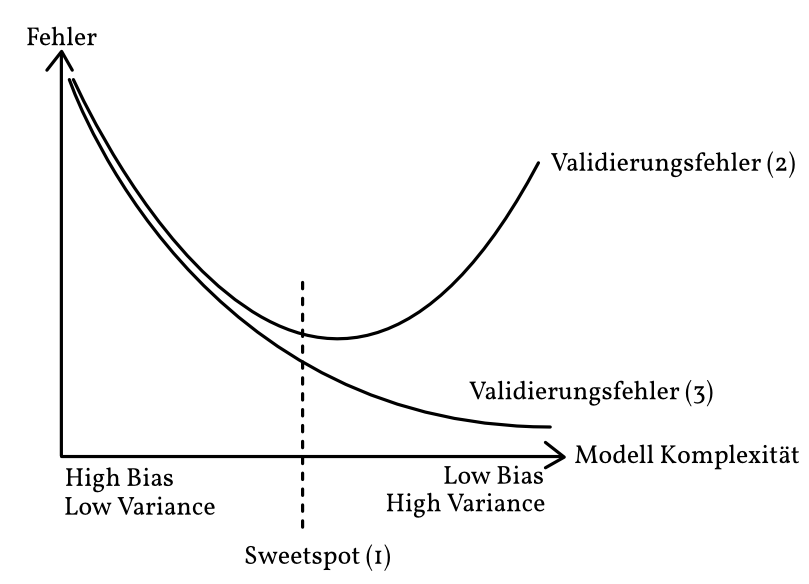
\includegraphics[width=9cm]{graphs/graph.png}  
\label{Modell_Komplexität}
\caption{(1) Sweetspot: Guter Tradeoff zwischen Bias und Varianz. Verschiebt sich nach rechts mit mehr Daten.  (2) Validierungsfehler: Messen der Fehler von $\hat{f}$ auf unabhängigen validierungsdaten $(x^{(x+1},y^{(m+1)}),...,(x^{(m+k)},y^{(m+k)})$  (3) Trainingsfehler: Messen des Fehlers von $f$ auf den Trainingsdaten $(x^{(1)},y^{(1)}),...,(x^{(m)},y^{(m)})$}

\end{figure}
